\chapter{Funzionalità}
\label{sec:funzionalita}

% TODO: METTI IMMAGINI
\section{Modulo di correzione}
Il sistema in cui il modulo di correzione è inserito si occupa di individuare, classificare e tracciare le entità presenti nello stream video ricavato dalla camera.
Con i dati ottenuti effettua poi, attraverso l'utilizzo di euristiche sperimentali, la rilevazione di anomalie.
Le anomalie trattate sono:
% TODO: standardizza
\begin{itemize}
    \item Cambio di corsia non permesso
    \item Traffico congestionato
    \item Attraversamento pedonale fuori dalle strisce 
    \item Veicolo al di fuori della strada (es. marciapiede) %ew
    \item Urto tra veicoli e tra veicolo e pedone
    \item Sosta non consentita
\end{itemize}
La corretta implementazione del modulo di correzione, che è posto come filtro tra la classificazione e il tracciamento delle entità, ha il fine di migliorare i risultati della rilevazione delle anomalie elencate sopra.

\begin{figure}
    \caption{Sistema di rilevazione di anomalie in funzione}
    \label{fig:anomalie}
    \centering
    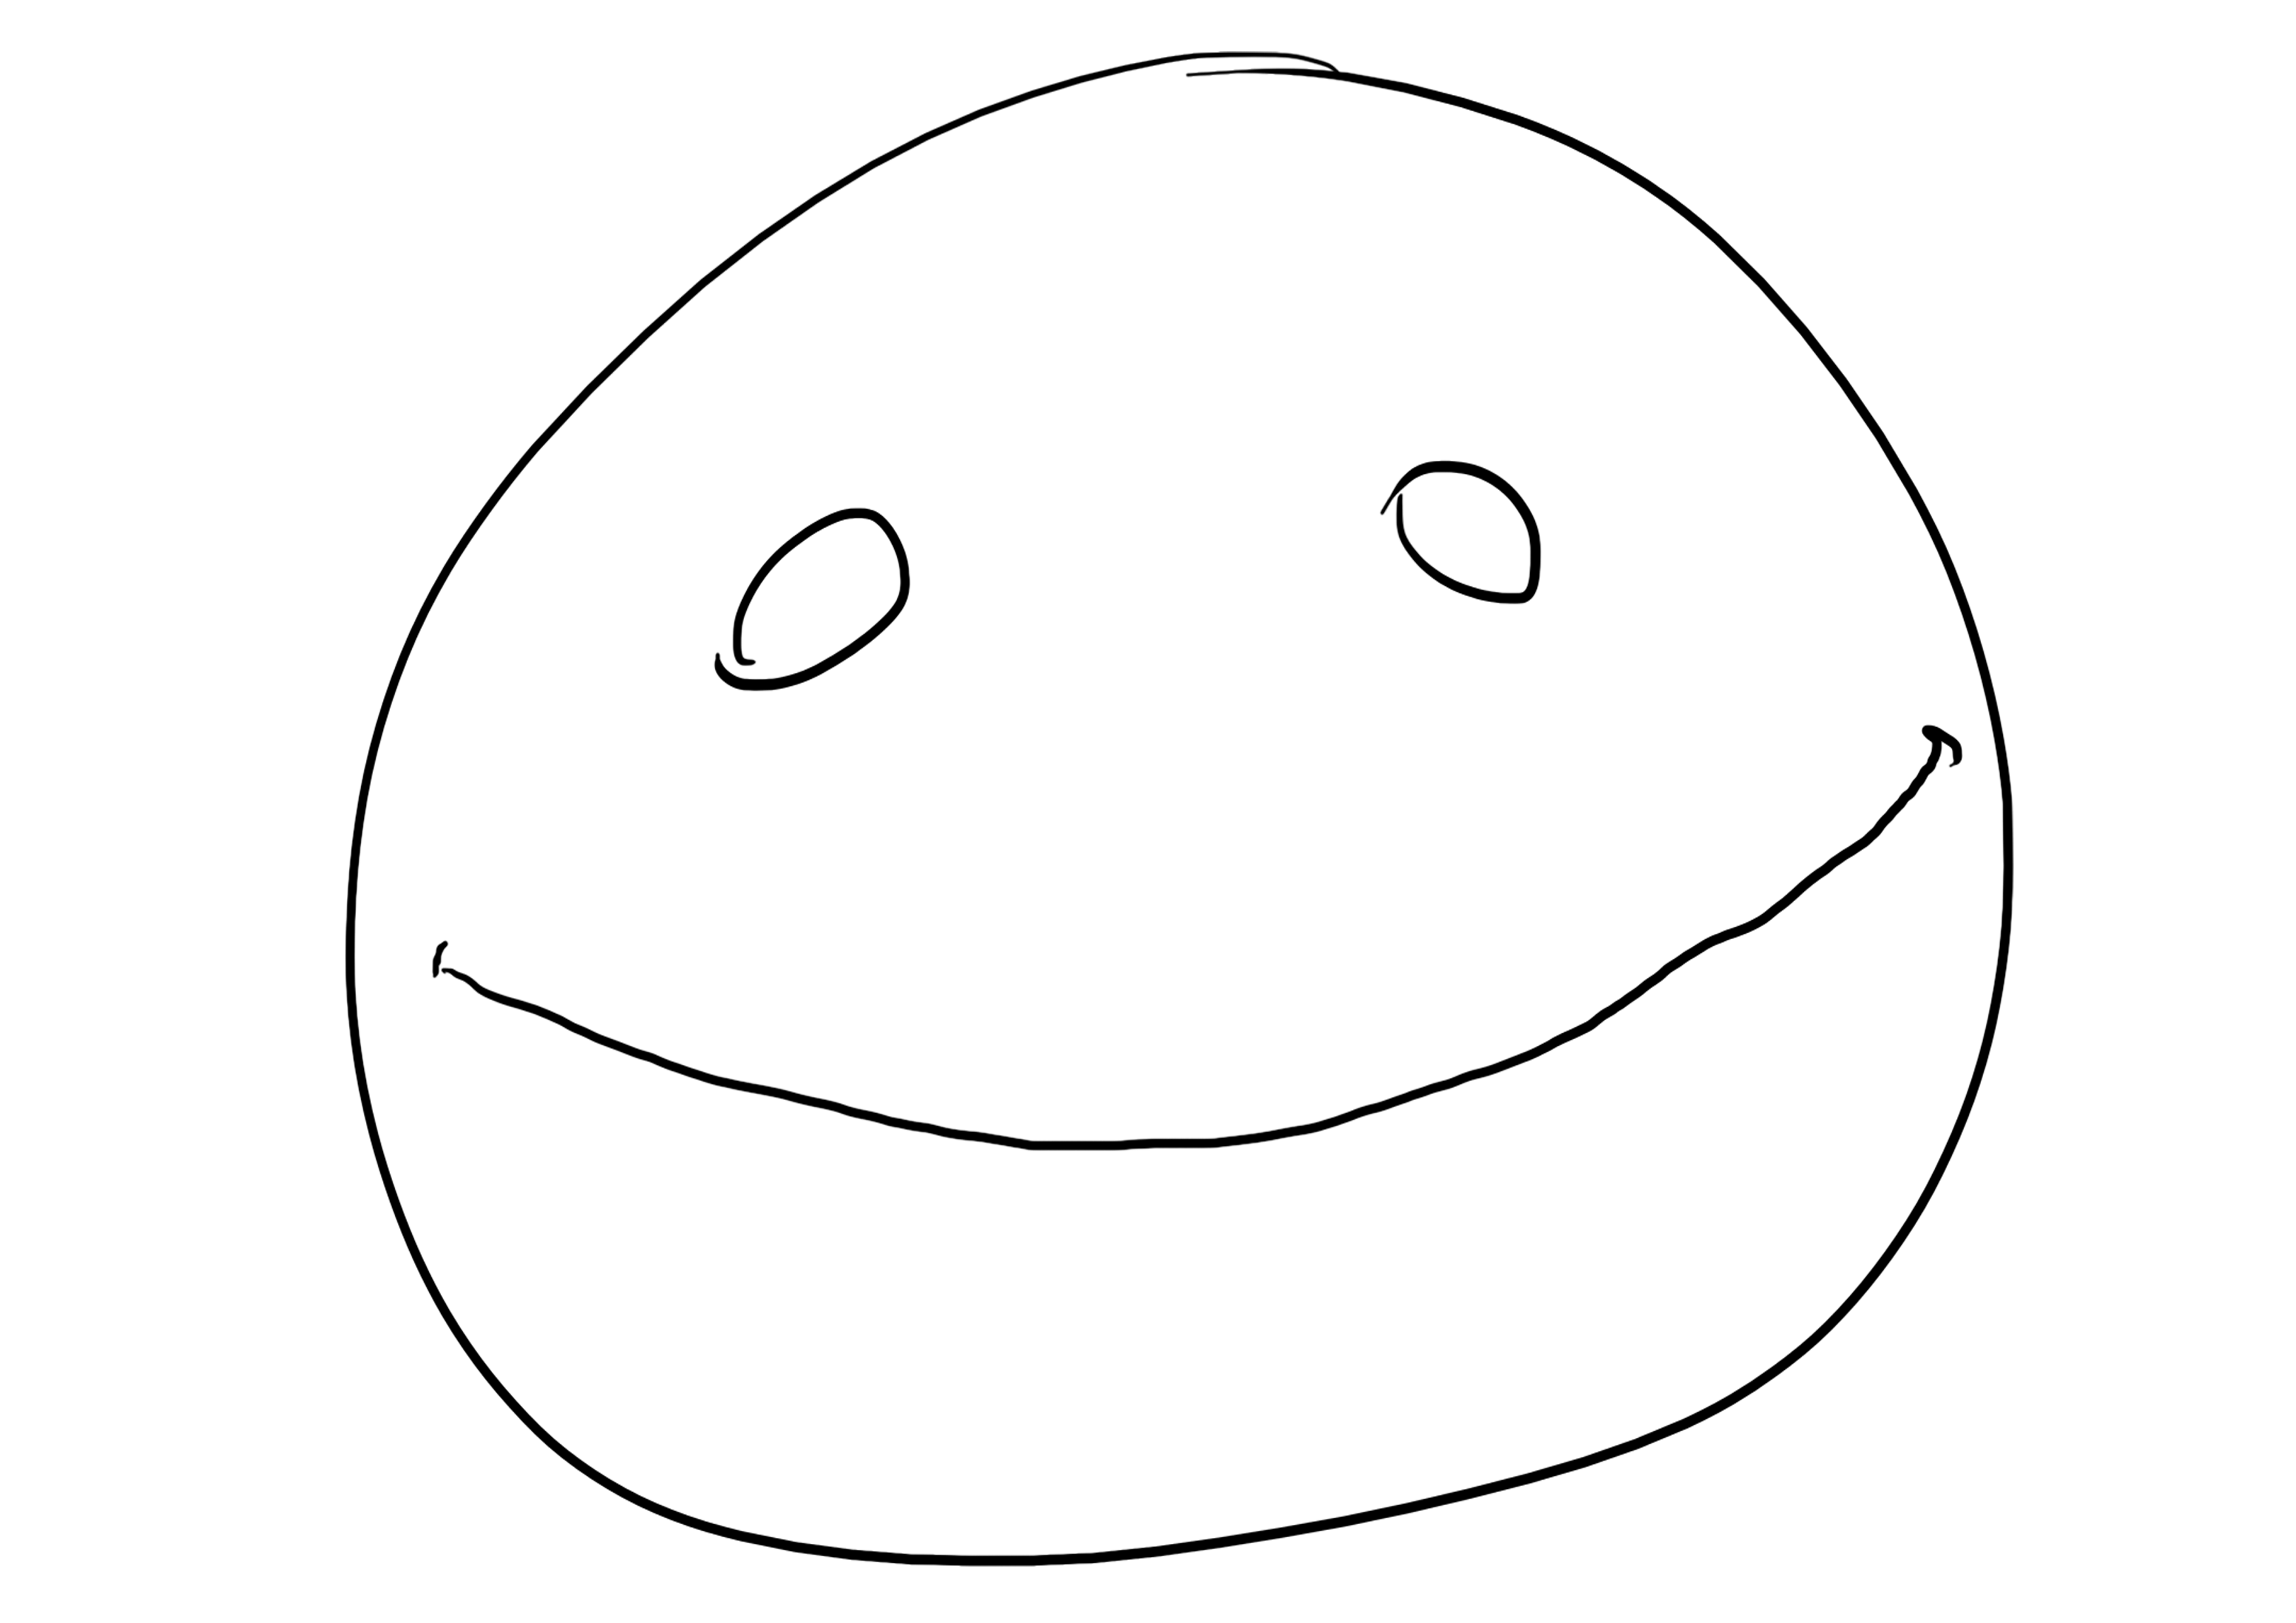
\includegraphics[width=.66\textwidth]{images/placeholder.png}
\end{figure}

\section{Strumento interattivo}
Lo strumento interattivo è sviluppato sulla base dell'ipotesi che l'operatore umano sia in grado di riconoscere un'immagine in cui non è presente la \emph{distorsione prospettica}, in quanto questa assomiglia a una ``vista dall'alto'', in cui le linee parallele e perpendicolari nella realtà appaiono parallele e perpendicolari. 
Linee disposte in questo modo sono comuni nell'ambito stradale.
Lo strumento fornisce quindi la possibilità di manipolare i parametri di \emph{lunghezza focale}, \emph{distanza tra piano e immagine (altezza)}, \emph{rotazione sull'asse x}, \emph{rotazione sull'asse y}.
Il primo è controllato attraverso la \emph{rotellina del mouse}, gli altri due con \emph{click \& drag} sull'immagine.
La \emph{rotazione sull'asse z} è raramente necessaria in situazioni reali e non è quindi manipolabile.

Lo strumento mostra una porzione dell'immagine dopo che la trasformazione è stata applicata.
L'operatore è quindi in grado di valutare la bontà della trasformazione visivamente.
Dato che la trasformazione non mantiene forma e dimensioni dell'immagine non è possibile applicare la trasformazione all'immagine e poi mostrarla.
Lo strumento quindi parte dalle coordinate dell'immagine già manipolata e per ogni pixel applica la trasformazione inversa.
Con le coordinate trovate va a copiare il pixel dell'immagine originale nella posizione trovata.
La trasformazione utilizzata per la manipolazione ha inoltre delle modifiche rispetto a quella indicata nel capitolo \ref{sec:teoria}: l'altezza utilizzata è fissata a 0 e la trasformazione viene traslata in modo da mantenere il punto centrale dell'immagine nella stessa posizione prima e dopo la trasformazione.
Senza queste modifiche la manipolazione dell'immagine risulta disorientante e difficile.

Sono presenti i controlli di navigazione relativi a \emph{zoom}, \emph{posizione x}, \emph{posizione y}.
Tutti i parametri, compresi quelli relativi a \emph{lunghezza focale} e \emph{rotazione}, sono modificabili con bottoni e campi testuali.
Una volta manipolata correttamente l'immagine è possibile salvare la matrice di trasformazione e i parametri configurati.
La matrice salvata, a differenza di quella della manipolazione, è generata usando anche \emph{l'altezza}.
Anche questa è traslata per mantenere il punto centrale dell'immagine originale nella stessa posizione.

Per migliorare i risultati è stato fornito un bottone che permette di visualizzare l'immagine originale.
È stata aggiunta anche una modalità di misurazione che permette di inserire segmenti che indicano la loro dimensione dopo la trasformazione.
Questi segmenti vengono manipolati visivamente insieme all'immagine ma le misure sono relative alla trasformazione che verrà poi salvata.

\begin{figure}
    \caption{Stumento interattivo: interfaccia}
    \label{fig:tool view}
    \centering
    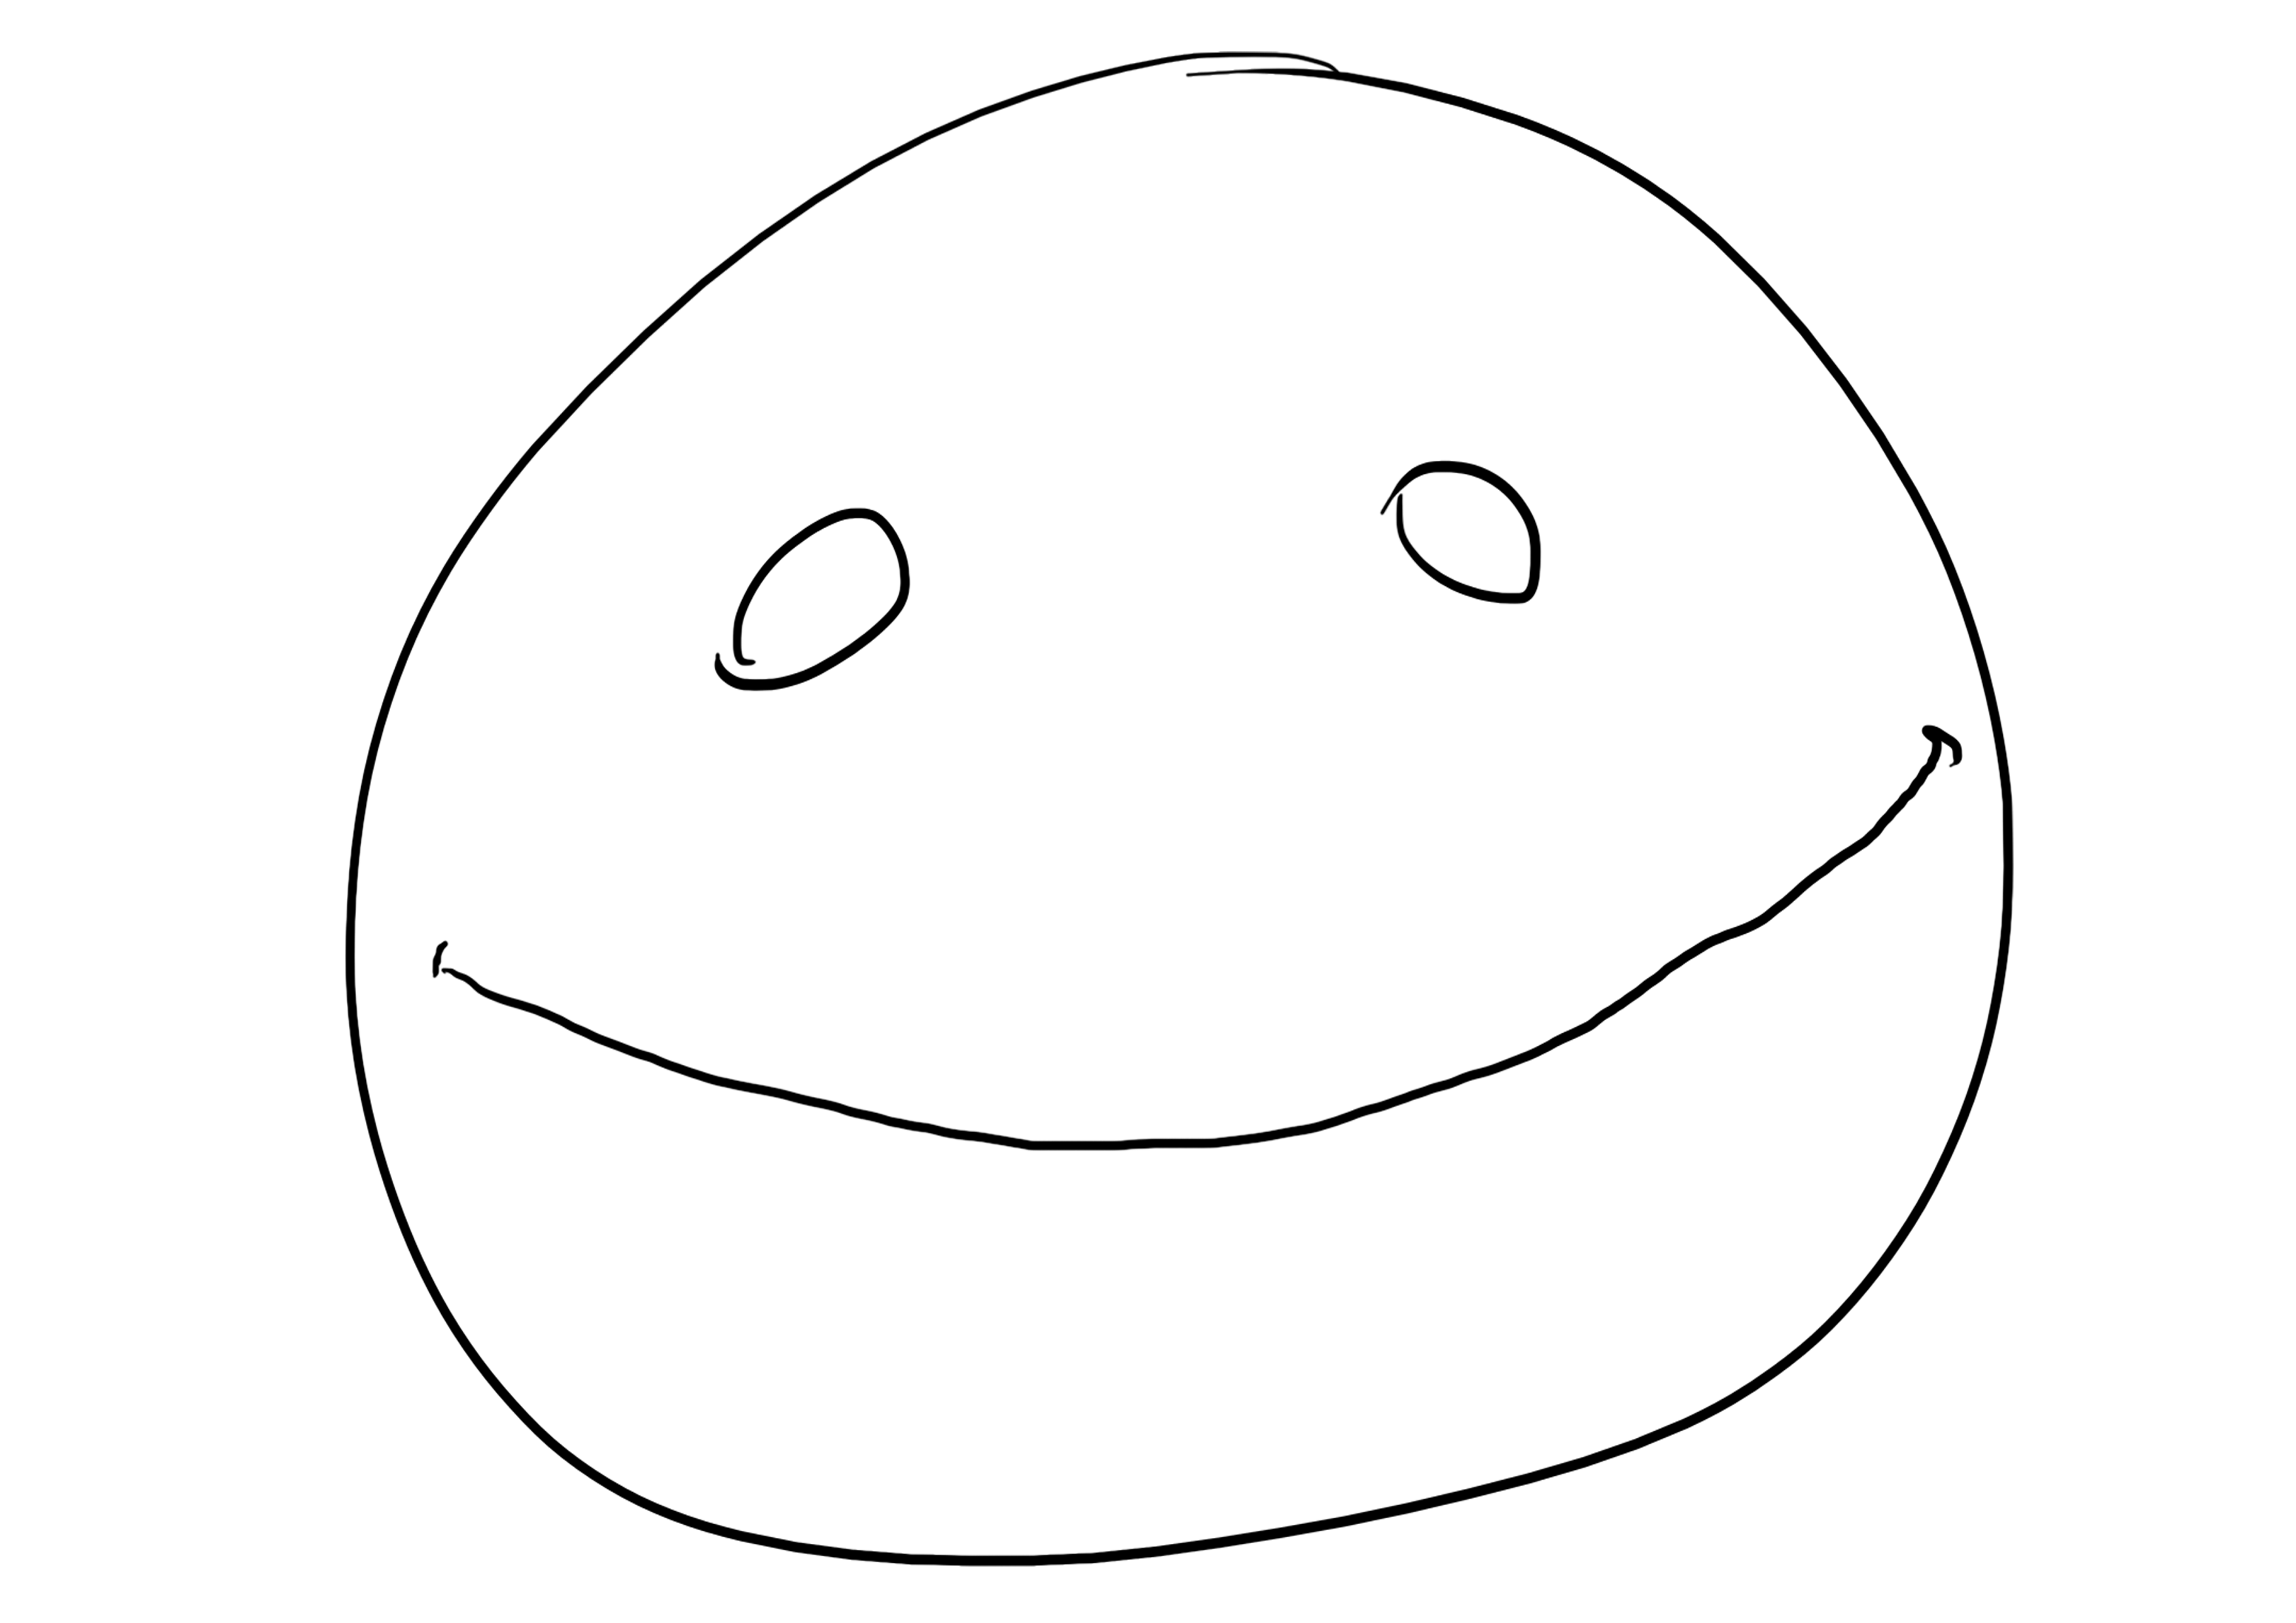
\includegraphics[width=.66\textwidth]{images/placeholder.png}
\end{figure}

\begin{figure}
    \caption{Stumento interattivo: modalità di misurazione}
    \label{fig:tool measure}
    \centering
    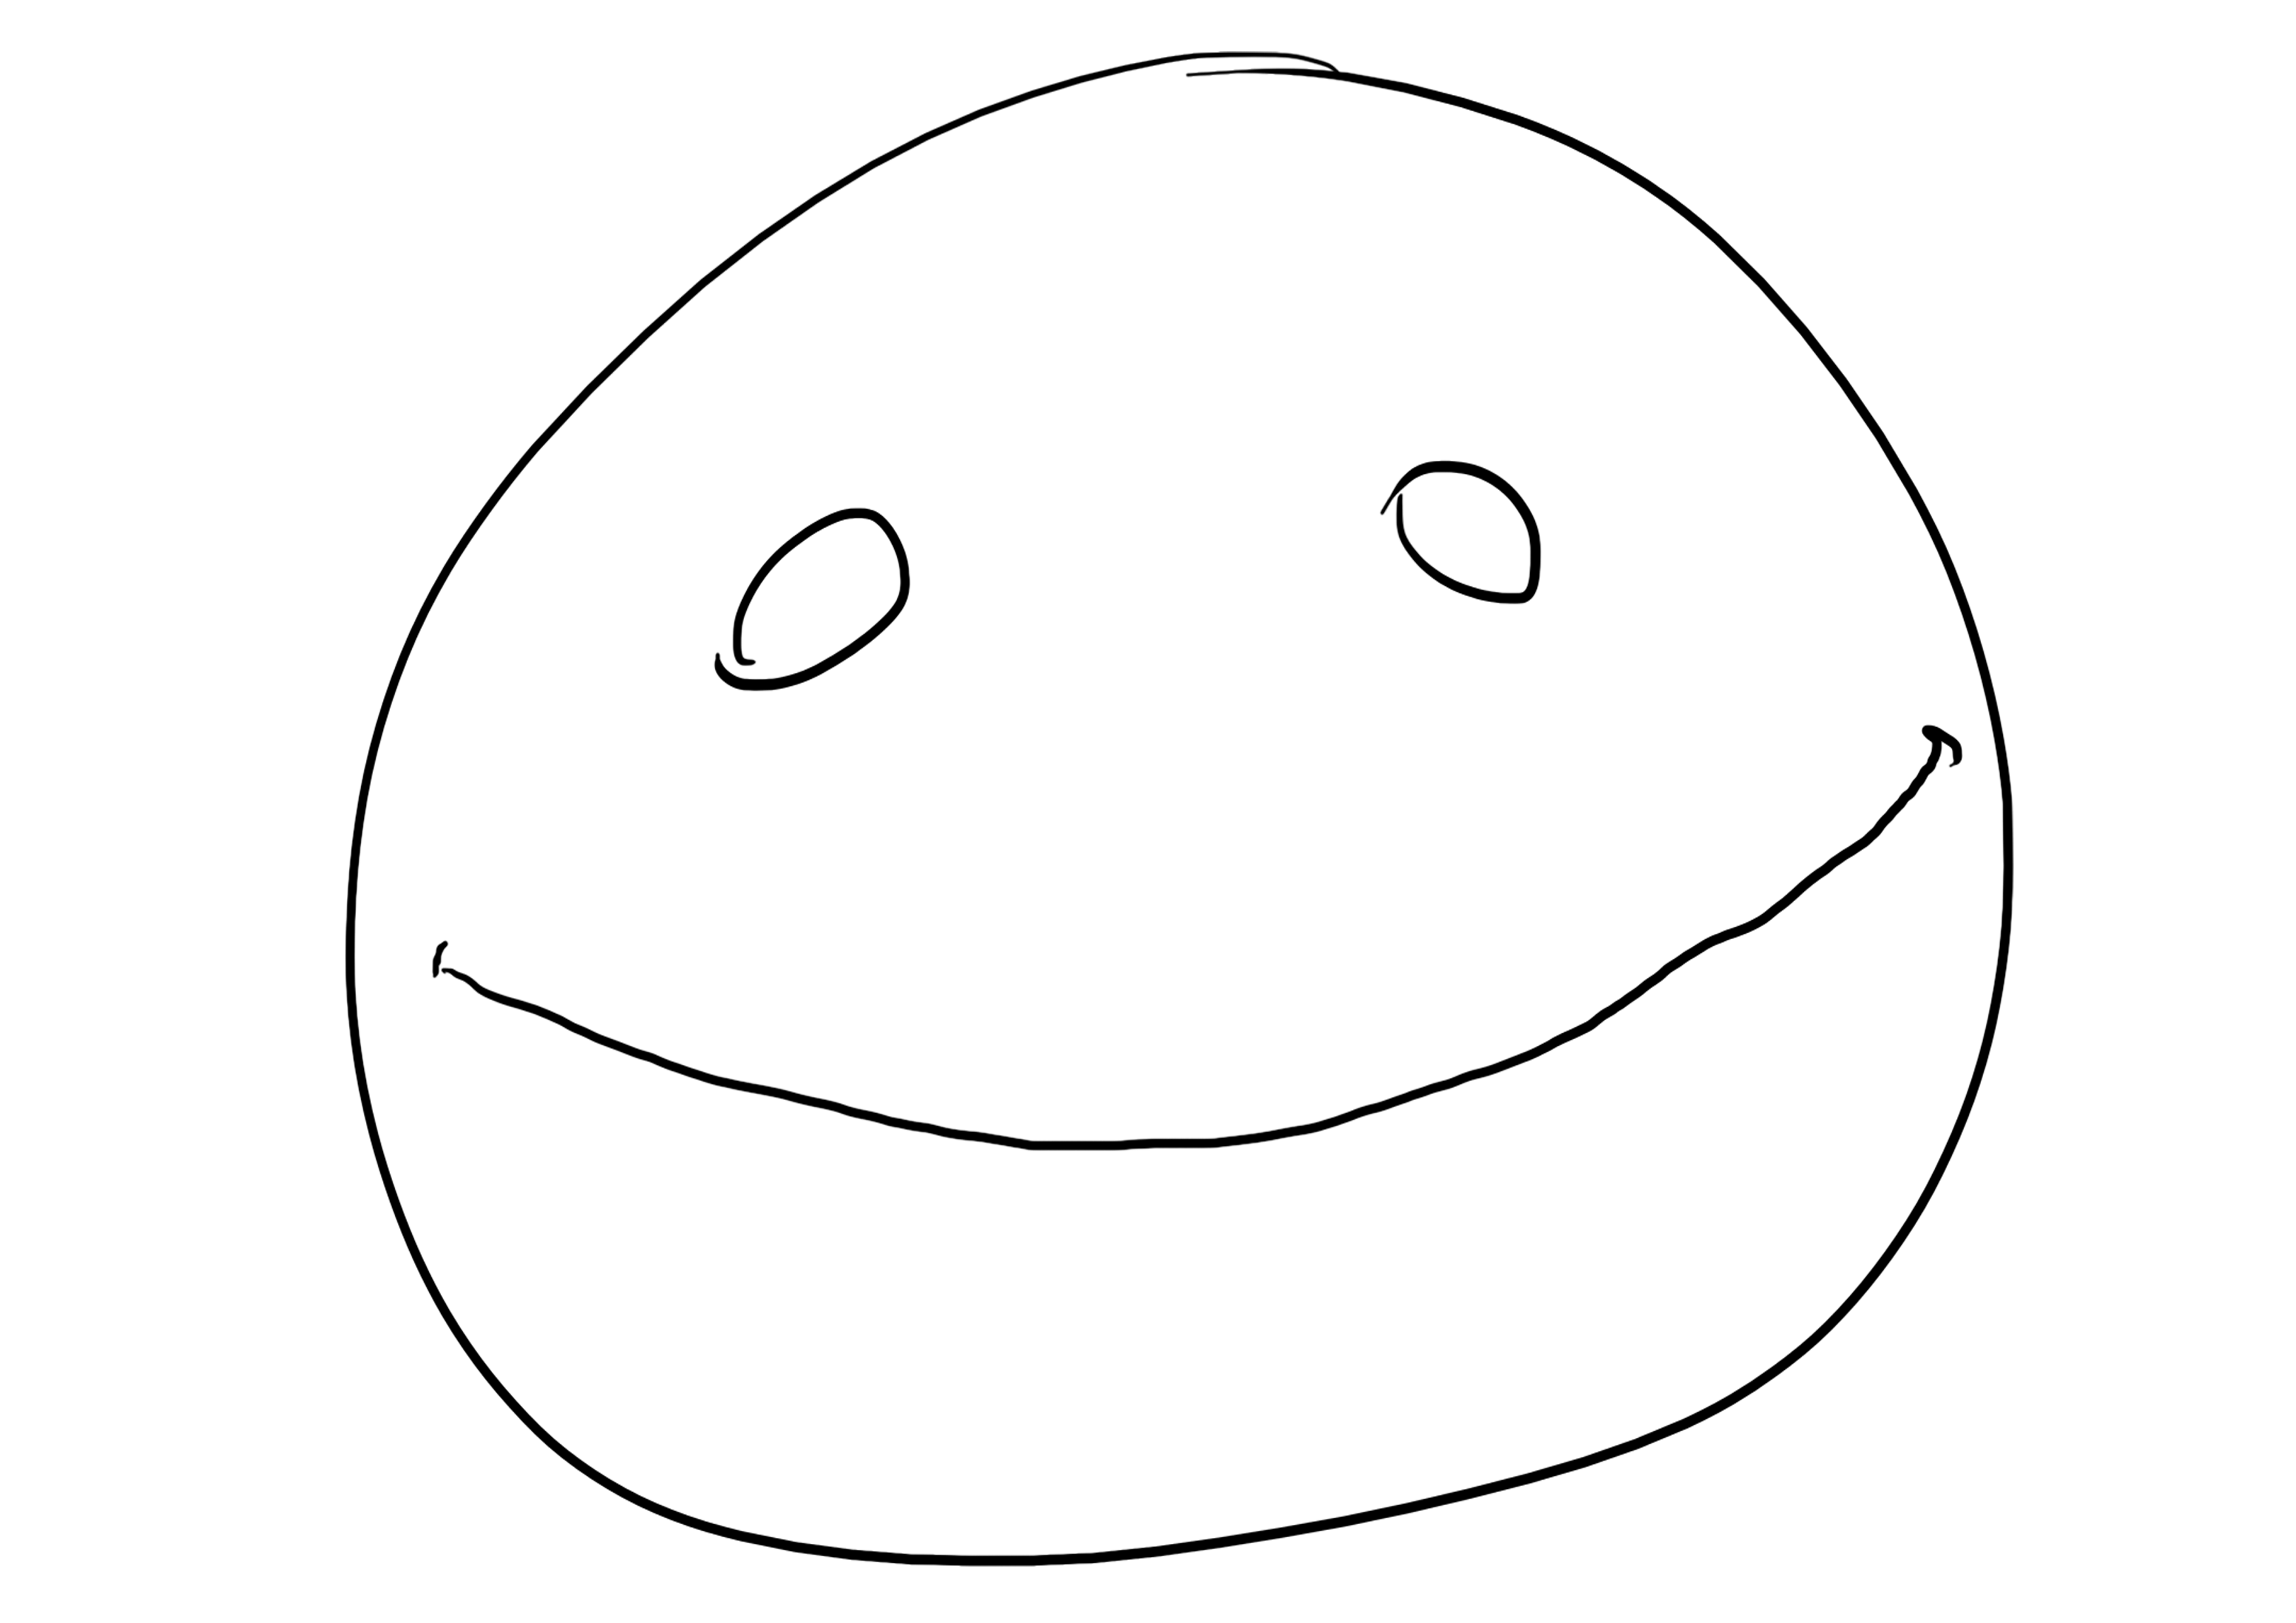
\includegraphics[width=.66\textwidth]{images/placeholder.png}
\end{figure}
